\section{Globaal ontwerp}  \label{sec:globaal}
Canvas.hs is een library die de programmeur kan importeren in zijn programma om er daarna met de API die Canvas.hs aanbiedt gemakkelijk een uitgebreide user interface mee te bouwen. Canvas.hs focust zich op elementaire input en geen ondersteuning hebben voor high level interface elementen zoals buttons en textarea's. Deze elementen zouden met behulp van Canvas.hs wel eenvoudig te implementeren moeten zijn.

\autoref{fig:overzicht_architectuur} geeft een overzicht van de architectuur. Canvas.hs bestaat uit een module en een client. De module is een library die de programmeur in zijn programma include. Bij het starten van de module start een HttpServer, een WebSocket-server en wordt de webpagina van de client automatisch gestart. De client bestaat uit een browserpagina met onder andere een canvas element. De module communiceert met de client via een WebSocket verbinding om grafische elementen op de canvas in de client te tekenen.

\begin{figure}
\begin{center}
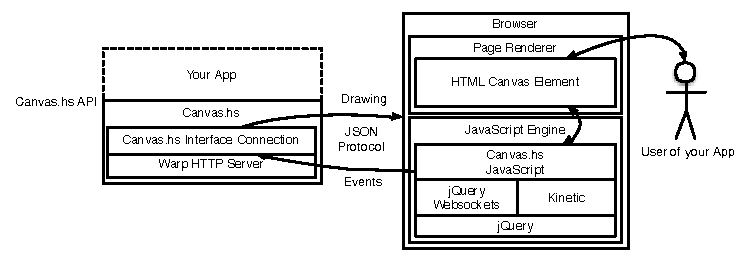
\includegraphics[keepaspectratio,width=\textwidth]{./images/architectuur_overzicht.pdf}
\caption{Overzicht van de architectuur van Canvas.hs}
\label{fig:overzicht_architectuur}
\end{center}
\end{figure}

-TODO: Overzicht geven van de architectuur
-TODO: Belangrijkste ontwerpkeuzes
-TODO: Concreet beeld geven van de output (voorbeeld)
-TODO: Plaatje van de Client